\documentclass{subfiles}

\begin{document}

    \chapter{Análisis y diseño}
    \label{chap:analisis_y_diseno}

        \section{Análisis de requisitos}
        \label{sec:analisis_de_requisitos}
        A continuación se enumerarán los requisitos del proyecto que se han obtenido a través de diferentes sesiones de estudio de diferentes productos similares en el mercado. A través de estos, se puede obtener una idea básica del producto a obtener.

        \subsection{Requisitos funcionales}
        \label{sec:requisitos_funcionales}

        Los requisitos funcionales son los casos prácticos que se implementarán en el sistema a través de distintas funcionalidades del mismo: desde respuestas al usuario hasta interacciones específicas con otros sistemas \cite{web:medium_requisitosfuncionalesynofuncionales}. En este proyecto se han identificado los siguientes:

%%%%%%%%%%%%%%%%%%%%%%%%%
%% REQUISITOS FUNCIONALES
%%%%%%%%%%%%%%%%%%%%%%%%%
\begin{longtblr}[
  caption = {Requisitos funcionales del sistema},
  label = {tab:requisitos_funcionales_del_sistema},
]{
  width = \linewidth,
  colspec = {Q[100]Q[842]},
  column{1} = {c},
  hlines,
  vlines,
}
\textbf{Código} & \textbf{Descripción}\\
RF01 & El sistema será capaz de obtener imágenes de la cámara de un dispositivo móvil\\
RF02 & El sistema será capaz de cargar modelos tridimensionales\\
RF03 & El sistema será capaz de insertar renderizaciones de modelos tridimensionales sobre otras imágenes\\
RF04 & El sistema será capaz de detectar el movimiento del dispositivo utilizado\\
RF05 & El sistema será capaz de iniciar una sesión de \ra \\
RF06 & El sistema será capaz de reproducir pistas de audio con efecto espacial\\
RF07 & El sistema será capaz de animar modelos tridimensionales\\
RF08 & El sistema será capaz de detectar superficies en imágenes captadas por el dispositivo móvil\\
RF09 & El sistema será capaz de ubicar figuras tridimensionales en superficies encontradas en imágenes\\
RF10 & El sistema será capaz de modificar la ubicación de una figura tridimensional\\
RF11 & El sistema será capaz de modificar la ubicación de un sonido espacial\\
RF12 & El sistema será capaz de modificar la orientación de la figura tridimensional en relación al movimiento del dispositivo\\
RF13 & El sistema será capaz de obtener modelos tridimensionales de una URL dada\\
RF14 & El sistema será capaz de cargar un modelo aleatorio de entre varios dados\\
RF15 & El sistema será capaz de detener la animación al cerrarse la sesión de \ra \\
RF16 & El sistema será capaz de detener la pista de audio reproducida al cerrarse la sesión de \ra
\end{longtblr}

%%%%%%%%%%%%%%%%%%%%%%%%%%%%%
%% FIN REQUISITOS FUNCIONALES
%%%%%%%%%%%%%%%%%%%%%%%%%%%%%

        \subsection{Requisitos no funcionales}
        \label{sec:requisitos_no_funcionales}

        A continuación se redactan los requisitos no funcionales del sistema, que son aquellas que definen propiedades del sistema en base a necesidades del usuario o a las restricciones del sistema \cite{web:medium_requisitosfuncionalesynofuncionales}. En este caso, se han encontrado los siguientes:

%%%%%%%%%%%%%%%%%%%%%%%%%%%%
%% REQUISITOS NO FUNCIONALES
%%%%%%%%%%%%%%%%%%%%%%%%%%%%
\begin{longtblr}[
  caption = {Requisitos no funcionales del sistema},
  label = {tab:requisitos_no_funcionales_del_sistema},
]{
  width = \linewidth,
  colspec = {Q[100]Q[842]},
  column{1} = {c},
  hlines,
  vlines,
}
\textbf{Código} & \textbf{Descripción}\\
RNF01 & El sistema deberá poder utilizarse en dispositivos móviles\\
RNF02 & El sistema deberá poder utilizarse en el sistema operativo \android \\
RNF03 & El sistema deberá poder utilizarse en el navegador \googlechrome para \android \\
RNF04 & El sistema deberá estar alojado en un servidor \linux \\
RNF05 & El sistema deberá ser accesible a través de un código QR\\
RNF06 & El sistema deberá cargar la \textit{landing page} en menos de 2 segundos\\
RNF07 & El sistema deberá cargar el modelo tridimensional en menos de 5 segundos
\end{longtblr}

%%%%%%%%%%%%%%%%%%%%%%%%%%%%%%%%
%% FIN REQUISITOS NO FUNCIONALES
%%%%%%%%%%%%%%%%%%%%%%%%%%%%%%%%

        \section{Casos de uso}
        \label{sec:casos_de_uso}
        Los casos de uso son descripciones de las distintas interacciones entre los diferentes actores (en este caso, el usuario) y el propio sistema \cite{web:uml2_5_1}. En este caso, el objetivo del actor será activar el sistema de \ra, <<jugar>> con él y escuchar la información que ofrece este mismo, por lo que podríamos obtener de aquí algunos casos de uso, que quedarán plasmados en la figura \ref{fig:analisis_casos_de_uso}:

        \begin{itemize}
            \item Iniciar sesión de \ra.
            \item Iniciar actividad de asistente virtual.
            \item Iniciar animación del modelo tridimensional.
            \item Iniciar pista de audio.
            \item Desplazar asistente virtual.
            \item Ubicar modelo tridimensional.
            \item Ubicar fuente de sonido de la pista de audio.
            \item Cerrar sesión de \ra.
        \end{itemize}

\begin{figure}[ht]
\centering
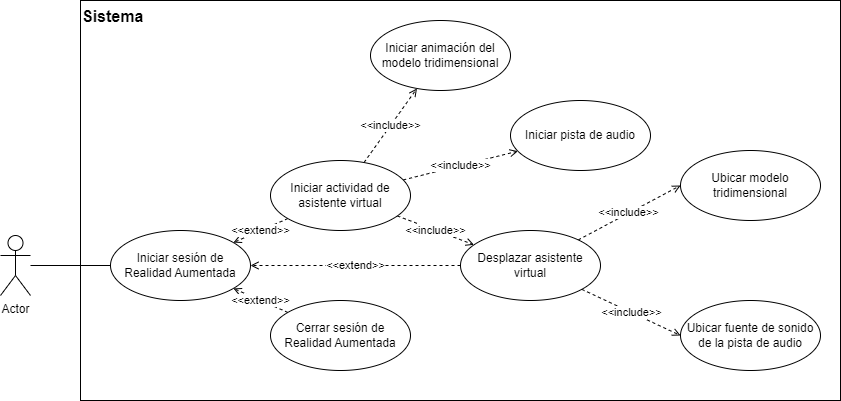
\includegraphics[width=0.9\textwidth]{img/analisis_casos_de_uso.png}
\caption{Diagrama de casos de uso.}
\label{fig:analisis_casos_de_uso}
\end{figure}

%%%%%%%%%%%%%%%%
%% CASO DE USO 1
%%%%%%%%%%%%%%%%

\begin{longtblr}[
  caption = {UC1: Iniciar sesión de \ra},
  label = {tab:iniciar_sesion_de_ra}
]{
  width = \linewidth,
  colspec = {Q[156]Q[698]},
  hlines,
  vlines,
}
\textbf{UC1} & \textbf{Iniciar sesión de \ra}\\
Descripción & El usuario lanza la sesión de \ra, haciendo que el sistema muestre las imágenes captadas por cámara y cargue los datos utilizados en dicha sesión\\
Precondición & El usuario ha entrado en la aplicación web\\
Extend & -\\
Include & -\\
Secuencia & {1. El sistema identifica el dispositivo utilizado como compatible y activa el botón <<Iniciar sesión de \textit{Realidad Aumentada}>>
\\2. El usuario pulsa
sobre el botón <<Iniciar sesión de \textit{Realidad Aumentada}>>
\\3. El sistema
muestra por la interfaz las imágenes captadas por la cámara del dispositivo
\\4. El sistema carga
los modelos tridimensionales
\\5. El sistema
detecta una superficie en las imágenes captadas por la cámara del dispositivo
\\6. El sistema
muestra un puntero sobre la superficie detectada}\\
Secuencia alternativa & {1A. El sistema identifica el dispositivo utilizado como no compatible y muestra un mensaje avisando al usuario.}
\end{longtblr}

%%%%%%%%%%%%%%%%
%% CASO DE USO 2
%%%%%%%%%%%%%%%%

\begin{longtblr}[
  caption = {UC2: Iniciar actividad de asistente virtual.},
  label = {tab:iniciar_actividad_de_asistente_virtual}
]{
  width = \linewidth,
  colspec = {Q[156]Q[698]},
  hlines,
  vlines,
}
\textbf{UC2} & \textbf{Iniciar actividad de asistente virtual}\\
Descripción & El usuario interactúa con el sistema y este muestra al asistente virtual moviéndose y hablando\\
Precondición & {El usuario ha iniciado la sesión de \ra\\
El sistema ha cargado el modelo tridimensional y la pista de audio\\
El sistema muestra un puntero sobre las superficies horizontales}\\
Extend & Iniciar sesión de \ra\\
Include & {Iniciar animación del modelo tridimensional\\
Iniciar pista de audio\\
Desplazar asistente virtual}\\
Secuencia & {1. El usuario apunta hacia una superficie horizontal\\
2. El usuario pulsa sobre la pantalla\\
3. El sistema oculta el puntero\\
4. El sistema coloca al asistente virtual donde antes estaba el puntero\\
5. El sistema arranca la animación del asistente virtual a la vez que la pista de audio\\
6. El sistema detiene la animación y la pista de audio al terminar ambos}
\end{longtblr}
\newpage

%%%%%%%%%%%%%%%%
%% CASO DE USO 3
%%%%%%%%%%%%%%%%

\begin{longtblr}[
  caption = {UC3: Iniciar animación del modelo tridimensional.},
  label = {tab:iniciar_animacion_del_modelo_tridimensional}
]{
  width = \linewidth,
  colspec = {Q[156]Q[698]},
  hlines,
  vlines,
}
\textbf{UC3} & \textbf{Iniciar animación del modelo tridimensional}\\
Descripción & El usuario interactúa con el sistema y este inicia la animación del modelo tridimensional\\
Precondición & {El usuario ha iniciado la sesión de \ra\\
El sistema ha cargado el modelo tridimensional y la pista de audio\\
El sistema muestra al modelo tridimensional estático en la \textit{Realidad Aumentada}}\\
Extend & -\\
Include & -\\
Secuencia & {1. El usuario pulsa sobre la pantalla\\
2. El sistema arranca la animación del asistente virtual\\
3. El sistema detiene la animación al terminar}
\end{longtblr}

%%%%%%%%%%%%%%%%
%% CASO DE USO 4
%%%%%%%%%%%%%%%%

\begin{longtblr}[
  caption = {UC4: Iniciar pista de audio.},
  label = {tab:iniciar_pista_de_audio}
]{
  width = \linewidth,
  colspec = {Q[156]Q[698]},
  hlines,
  vlines,
}
\textbf{UC4} & \textbf{Iniciar pista de audio.}\\
Descripción & El usuario interactúa con el sistema y este inicia la animación del modelo tridimensional\\
Precondición & {El usuario ha iniciado la sesión de \ra\\
El sistema ha cargado el modelo tridimensional y la pista de audio}\\
Extend & -\\
Include & -\\
Secuencia & {1. El usuario pulsa sobre la pantalla\\
2. El sistema arranca la animación del asistente virtual\\
3. El sistema detiene la animación al terminar}
\end{longtblr}

%%%%%%%%%%%%%%%%
%% CASO DE USO 5
%%%%%%%%%%%%%%%%

\begin{longtblr}[
  caption = {UC5: Desplazar asistente virtual.},
  label = {tab:desplazar_asistente_virtual}
]{
  width = \linewidth,
  colspec = {Q[156]Q[698]},
  hlines,
  vlines,
}
\textbf{UC5} & \textbf{Desplazar asistente virtual}\\
Descripción & El usuario interactúa con el sistema y este muestra al asistente virtual en una nueva localización. El sonido se origina desde el mismo lugar en el que está el asistente\\
Precondición & {El usuario ha iniciado la sesión de \ra\\
El sistema ha cargado el modelo tridimensional y la pista de audio\\
El sistema muestra las imágenes captadas por la cámara}\\
Extend & -\\
Include & {Ubicar modelo tridimensional\\
Ubicar fuente de sonido de la pista de audio}\\
Secuencia & {1. El sistema muestra al asistente en la \ra\\
2. El usuario pulsa sobre la pantalla apuntando con la cámara a un lugar donde no está el asistente\\
3. El sistema emplaza al asistente en la nueva posición, ubicando también en la nueva posición el origen del sonido}\\
Secuencia alternativa & {1A. El sistema muestra el puntero en la \ra\\
2A. El usuario pulsa sobre la pantalla apuntando con la cámara y el puntero\\
3A. El sistema hace aparecer al asistente en la nueva posición, ubicando también en la nueva posición el origen del sonido y ocultando el puntero}
\end{longtblr}

%%%%%%%%%%%%%%%%
%% CASO DE USO 6
%%%%%%%%%%%%%%%%

\begin{longtblr}[
  caption = {UC6: Ubicar modelo tridimensional.},
  label={tab:ubicar_modelo_tridimensional}
]{
  width = \linewidth,
  colspec = {Q[156]Q[698]},
  hlines,
  vlines,
}
\textbf{UC6} & \textbf{Ubicar modelo tridimensional}\\
Descripción & El usuario interactúa con el sistema y este modifica la ubicación del modelo tridimensional\\
Precondición & {El usuario ha iniciado la sesión de \ra\\
El sistema ha cargado el modelo tridimensional y la pista de audio\\
El sistema muestra un puntero sobre las superficies horizontales}\\
Extend & -\\
Include & {-}\\
Secuencia & {1. El sistema muestra al modelo tridimensional en la \ra\\
2. El usuario pulsa sobre la pantalla apuntando con la cámara a un lugar donde no está el modelo tridimensional\\
3. El sistema emplaza al modelo en la nueva posición}\\
Secuencia alternativa & {1A. El sistema muestra el puntero en la \ra\\
2A. El usuario pulsa sobre la pantalla apuntando con la cámara y el puntero\\
3A. El sistema emplaza al modelo en la nueva posición, ocultando el puntero}
\end{longtblr}
\newpage

%%%%%%%%%%%%%%%%
%% CASO DE USO 7
%%%%%%%%%%%%%%%%

\begin{longtblr}[
  caption = {UC7: Ubicar fuente de sonido de la pista de audio},
  label = {tab:ubicar_fuente_de_sonido_de_la_pista_de_audio}
]{
  width = \linewidth,
  colspec = {Q[156]Q[698]},
  hlines,
  vlines,
}
\textbf{UC7} & \textbf{Ubicar fuente de sonido de la pista de audio}\\
Descripción & El usuario interactúa con el sistema y este modifica la ubicación de la fuente de sonido\\
Precondición & {El usuario ha iniciado la sesión de \ra\\
El sistema ha cargado el modelo tridimensional y la pista de audio\\
El sistema muestra las imágenes captadas por la cámara}\\
Extend & -\\
Include & {-}\\
Secuencia & {1. El sistema reproduce la pista de audio con el origen del sonido ubicado en un lugar específico\\
2. El usuario pulsa sobre la pantalla apuntando con la cámara a un lugar distinto\\
3. El sistema emplaza el origen del sonido en la nueva posición}\\
Secuencia alternativa & {1A. El sistema mantiene la pista de audio a la espera de ser reproducida\\
2A. El usuario pulsa sobre la pantalla apuntando con la cámara a un lugar específico\\
3A. El sistema comienza la reproducción de la pista ubicando el origen del sonido en la posición indicada por el usuario}
\end{longtblr}

%%%%%%%%%%%%%%%%
%% CASO DE USO 8
%%%%%%%%%%%%%%%%

\begin{longtblr}[
  caption = {UC8: Cerrar sesión de \ra.},
  label = {tab:cerrar_sesion_de_ra}
]{
  width = \linewidth,
  colspec = {Q[156]Q[698]},
  hlines,
  vlines,
}
\textbf{UC8} & \textbf{Cerrar sesión de \ra}\\
Descripción & El usuario pulsa el botón de volver para salir de la sesión de \ra\\
Precondición & {El usuario ha iniciado la sesión de \ra}\\
Extend & Iniciar sesión de \ra\\
Include & {-}\\
Secuencia & {1. El usuario pulsa dos veces seguidas el botón <<volver>> del dispositivo móvil\\
2. El sistema detiene la animación del modelo y la reproducción del audio\\
3. El sistema devuelve al usuario a la \textit{landing page}}
\end{longtblr}

%%%%%%%%%%%%%%%%%%%
%% FIN CASOS DE USO
%%%%%%%%%%%%%%%%%%%

        \section{Estructura}
        \label{sec:estructura}
        Debido a la clara repartición de tareas en cada sección del código, se ha pretendido aplicar una separación tipo Modelo-Vista-Controlador en la aplicación, de manera que todo esté visiblemente separado y se pueda utilizar un sistema de orientación a objetos en toda la parte escrita en \js.

        \paragraph{}
        La primera sección a comentar sería el Modelo. En esta aplicación, tal y como se ha planteado el desarrollo y teniendo en cuenta qué librerías externas se han incorporado y cómo se han utilizado, se ha tratado a estas como si fueran el propio Modelo. Así, nuestra información es en sí las librerías externas añadidas, que serán además las que se encarguen de cargar los datos estáticos de servidor: los modelos en 3D y las grabaciones de las voces de estos.

        \paragraph{}
        La segunda sección sería la Vista. En este caso, la Vista de esta aplicación constaría únicamente de un HTML llamado \textit{index}, que sería además la \textit{landing page} de la aplicación. Sobre esta misma página será sobre la que se colocará más tarde un \textit{<<canvas>>}, que es el elemento HTML que permite mostrar elementos gráficos de manera dinámica a través de \js. Utilizando este último podremos mostrar las imágenes captadas a través de la cámara del dispositivo móvil y mezclarlas con los modelos en 3D para generar nuestra \ra.

        \paragraph{}
        Por último, la sección restante sería el Controlador. En este, se procesan todos los eventos generados por el usuario, además de tratar toda la información que se recibirá de los sensores del dispositivo para poder generar las imágenes de manera verosímil. En este se ubicará un bucle que se ocupará de obtener la imagen a mostrar, mezclarla con el modelo en 3D, renderizar la imagen y situarla en la vista, todo esto de la manera más fluida posible para que el espectador no tenga impresiones que entorpezcan la experiencia de usuario.

        \paragraph{}
        Además, esta almacenará también información de la Sesión necesaria para el correcto procesamiento del sistema, tales como los modelos en 3D cargados, la referencia al objeto de \js con el \textit{<<canvas>>} antes mencionado, la posición del usuario y otros datos necesarios para el funcionamiento del sistema que serán mencionados a lo largo de esta memoria.

        \paragraph{}
        Es importante mencionar que, a pesar de que se ha tratado a este sistema como un Modelo-Vista-Controlador y se le ha presentado como tal, sería más justo tratar a la aplicación como si utilizara el patrón Modelo-Vista-Presentador \cite{web:mvp} por varias razones.

        \paragraph{}
        La primera es que no tenemos constancia de cómo almacenan estas librerías las pocas referencias que se le entregan a la Vista y, aún manteniendo esta referencia como si lo tratara como la Vista en este tipo de patrones, no parece realizar cambios sobre esta de manera directa.

        \paragraph{}
        La segunda es que las actualizaciones se realizan directamente desde el Controlador, siendo necesario realizar desde este último acciones explícitas para actualizar la apariencia de la vista, como por ejemplo el renderizado de la imagen a mostrar en pantalla.

        \paragraph{}
        Por último y más importante, es necesario que todos los cambios estén revisados en el bucle que se genera en el Controlador, el cual se tratará más adelante. Esto obliga a este último a solicitar información continuamente a las librerías, hacer cálculos y mostrarlos en pantalla, mientras está atento a los eventos de los usuarios.

        \begin{figure}
        \centering
        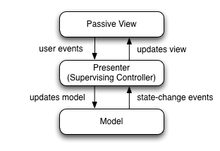
\includegraphics[width=0.5\textwidth]{img/mvp.png}
        \caption[Representación gráfica del patrón Modelo-Vista-Presentador.]{Representación gráfica del patrón Modelo-Vista-Presentador. Fuente: \citetitle{web:wikipedia_modelviewpresenter}.}
        \label{fig:mvp}
        \end{figure}

        \paragraph{}
        Por todo esto, y dado que la lógica de negocio está separada de la interfaz de usuario, la estructura se corresponde con el patrón Modelo-Vista-Presentador. Sin embargo, dado que desde el inicio del proyecto se trató cada parte como el clásico Modelo-Vista-Controlador, y dado que el Modelo-Vista-Presentador proviene de este último, cada parte será nombrada como si lo fuera, aún siendo conscientes de las diferencias.

        \paragraph{}
        Cabe destacar que el patrón Modelo-Vista-Presentador, al igual que el Modelo-Vista-Controlador, implementa en cierto modo el patrón \textit{Observer} \cite{book:gamma_erich_patronesdediseno}, que define una dependencia de forma que cuando un objeto cambie de estado se notifica y se actualizan automáticamente todos los objetos que dependen de él. En este caso, la vista actuaría a modo de Observador, lanzando las acciones adecuadas para que se actualice el Modelo del sistema.

        \section{Modelo de dominio}
        \label{sec:modelo_de_dominio}
%%%%%%%%%%%%%%%%%%%%%
%% DIAGRAMA DE CLASES
%%%%%%%%%%%%%%%%%%%%%
\begin{figure}[ht]
\centering
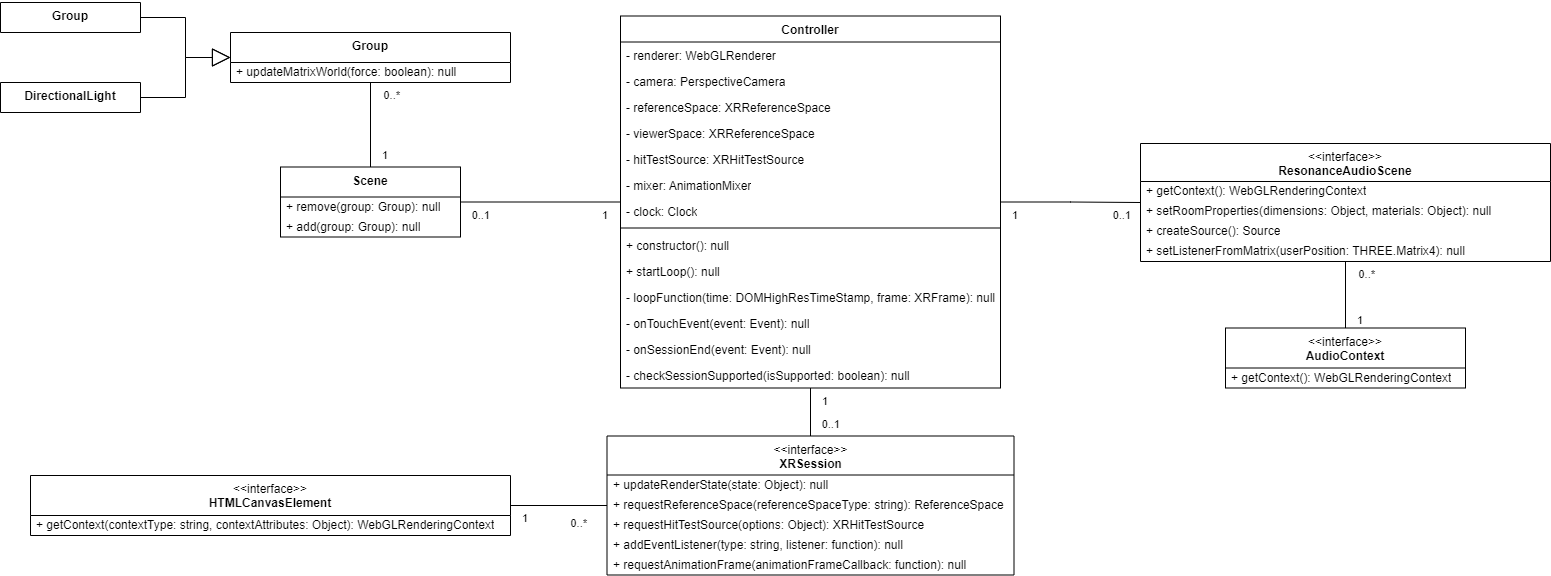
\includegraphics[width=0.9\textwidth]{img/analisis_modelo_de_dominio.png}
\caption{Modelo de dominio.}
\label{fig:analisis_modelo_de_dominio}
\end{figure}
        El proyecto \titlename consta, en verdad, de un modelo de dominio muy sencillo, al mantener centralizada la funcionalidad en el controlador, tal y como se comentó en la sección anterior. Por ello, el apartado más complejo se encuentra en este, siendo todo lo demás mucho más sencillo. El modelo, por otro lado, está formado por las interfaces de las herramientas externas utilizadas mencionadas en la sección \ref{sec:herramientas_de_ra}. La vista se controla a su vez a través de la interfaz \textit{HTMLCanvasElement} proporcionada por \js.



%%%%%%%%%%%%%%%%%%%%%%%%%%%%%%%%%
%% DIAGRAMA DE COMPONENTES
%%%%%%%%%%%%%%%%%%%%%%%%%%%%%%%%%
        \section{Diagrama de componentes}
        \label{sec:diagrama_de_componentes}

Mediante el diagrama de componentes, podemos ver que gran parte del sistema se basa en el uso de herramientas externas, las cuáles han implicado un estudio profundo para implicarlas de la manera correcta en la aplicación.

\begin{figure}[ht]
\centering
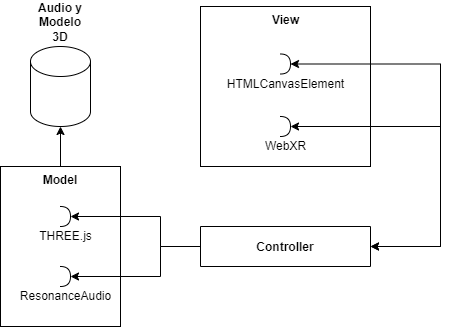
\includegraphics[width=0.75\textwidth]{img/analisis_diagrama_de_componentes.png}
\caption{Diagrama de componentes.}
\label{fig:analisis_diagrama_de_componentes}
\end{figure}

%%%%%%%%%%%%%%%%%%%%%%%%%
%% DIAGRAMA DE DESPLIEGUE
%%%%%%%%%%%%%%%%%%%%%%%%%
        \section{Diagrama de despliegue}
        \label{sec:diagrama_de_despliegue}
        
El diagrama de despliegue muestra la relación entre los diferentes elementos de software y el hardware que los contiene. En este caso, al ser una aplicación web, la comunicación está planteada para que se impliquen en todo momento navegadores (en nuestro caso, específicamente el navegador \googlechrome para dispositivos \android) con el servidor \aws.

\begin{figure}[ht]
\centering
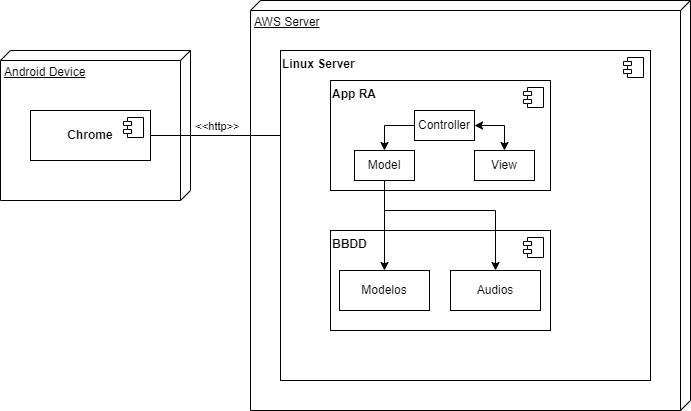
\includegraphics[width=0.95\textwidth]{img/analisis_diagrama_de_despliegue.png}
\caption{Diagrama de despliegue.}
\label{fig:analisis_diagrama_de_despliegue}
\end{figure}

%%%%%%%%%%%%%%%%%%%%%%%%%%%%%%%%%
%% DIAGRAMA DE MAQUINAS DE ESTADO
%%%%%%%%%%%%%%%%%%%%%%%%%%%%%%%%%
\newpage
        \section{Diagrama de máquinas de estado}
        \label{sec:diagrama_de_maquinas_de_estado}
        
El asistente virtual, dentro de la sesión de \ra, tiene un comportamiento básico y reproducible que puede verse reflejado en el diagrama de máquinas de estado, que a su vez deja ver la relación entre estos comportamientos y la interacción del usuario.

\begin{figure}[ht]
\centering
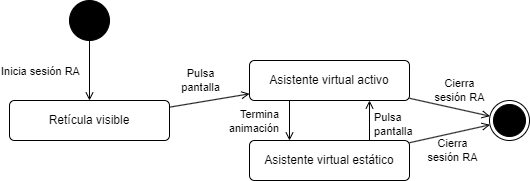
\includegraphics[width=0.95\textwidth]{img/analisis_diagrama_maquinas_de_estado.png}
\caption{Diagrama de máquinas de estado.}
\label{fig:analisis_diagrama_maquinas_de_estado}
\end{figure}

%%%%%%%%%%%%%%%%%%%%%%%%%%
%% DIAGRAMA DE ACTIVIDADES
%%%%%%%%%%%%%%%%%%%%%%%%%%
        \section{Diagrama de actividades}
        \label{sec:diagrama_de_actividades}
        
Para relatar la manera en que se ejecutaría un flujo básico, se muestra también un diagrama de actividades con la forma más normal en que se ejecutaría la aplicación.

\begin{figure}[ht]
\centering
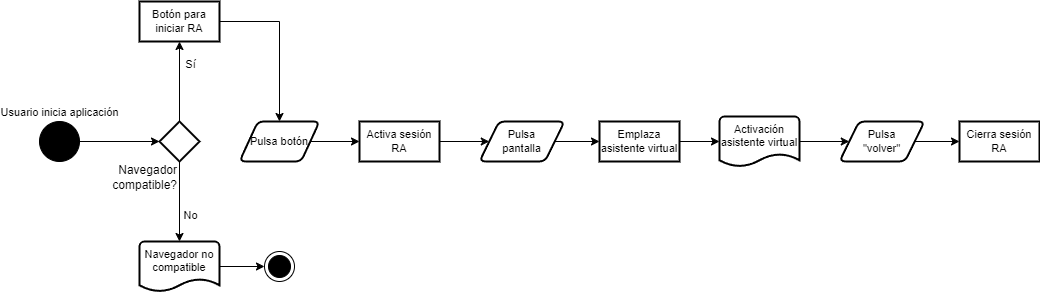
\includegraphics[width=0.95\textwidth]{img/analisis_y_diseno_diagrama_de_actividades.png}
\caption{Diagrama de actividades.}
\label{fig:analisis_y_diseno_diagrama_de_actividades}
\end{figure}

\end{document}